\chapter{Diseño de Pacmania}

En éste último capítulo de proyecto, se da una visión general de las actividades que componen el videojuego para tener una visión global de su diseño. Después se explica en profundidad el contenido del directorio que contiene los ficheros de configuración necesarios en el videojuego, especificando su formato y cómo han sido creados. Por último, se comentarán cada una de las actividades de la aplicación, completado de ésta forma la explicación del diseño del videojuego.

\newpage

\section{Visión General}

Toda aplicación realizada en Android está compuesta por las actividades, por lo que la forma más coherente de explicar cómo se ha desarrollado, es explicando las actividades que lo componen y la relación existente entre las mismas. Una forma de verlo de forma esquemática es mediante el diagrama de navegación entre actividades, junto con una breve descripción de cada una de ellas.
\newline

\begin{figure}[h!]
	\centering
          \includegraphics[width=14cm]{img/screenshot/workflow.jpg}
	\caption{Navegación entre Actividades}
\end{figure}

\begin{itemize}
\item \textbf{Boot:} primera actividad de la aplicación donde se carga la información común a todas las actividades en el contexto.
\item \textbf{Pacman:} comienza una vez finalizada la carga del contexto y contempla el menú general de la aplicación.
\item \textbf{Preferences:} muestra un listado con los distintos parámetros configurables en el videojuego.
\item \textbf{Scores:} muestra un listado con las diez mejores puntuaciones que los jugadores han obtenido en el videojuego.
\item \textbf{StartGame:} accesible desde la actividad principal y permite iniciar una nueva partida, mostrando inicialmente los distintos niveles disponibles.
\item \textbf{StarLevel:} se corresponde con un escenario del juego. Esta actividad es iniciada tras seleccionar en la actividad StartGame el nivel en el cual se desea jugar.
\item \textbf{VideoPresentantion:} muestra un video correspondiente a un escenario.
\end{itemize}

El nombre de la primera actividad al iniciar la aplicación es Boot. Su objetivo es cargar la información del contexto de la aplicación, mostrando mensajes e informando si todo funciona correctamente o no. Para poder explicar el comportamiento interno de esta actividad, se hará hincapié en la estructura de directorios del videojuego, llamada  \textbf{PacmanConfig},  donde se guarda la información necesaria para el proceso de carga de la aplicación.

\section{PacmanConfig}

Durante la ejecución del videojuego existe una gran cantidad de datos que han de ser recuperados del sistema de ficheros, algunos de estos ejemplos son las vídeos, sonidos, melodías,  texturas\ldots
El nombre por defecto de este directorio es PacmanConfig y se encuentra ubicado, por defecto, en el directorio principal de la tarjeta SD. La estructura de directorios de la que está compuesta es la siguiente:

\begin{figure}[h]
\centering
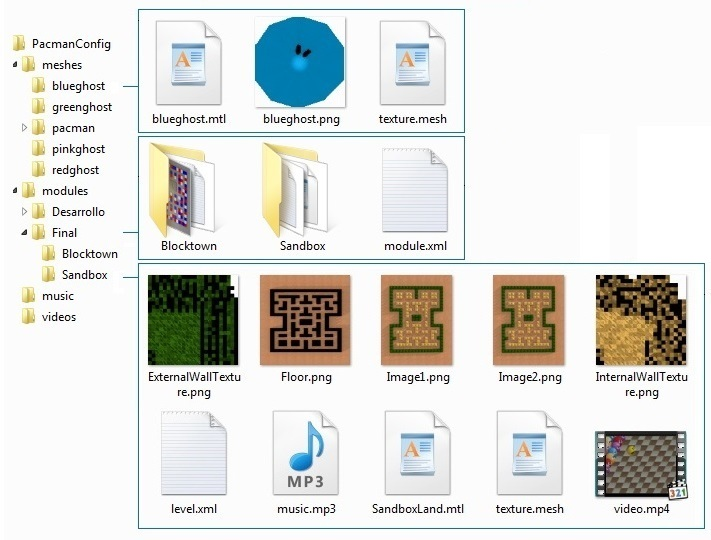
\includegraphics[width=14cm]{img/EstructuraPacmanConfig.jpg}	
\caption{Estructura del directorio de configuración del Pacman}
\end{figure}

\begin{itemize}
\item \textbf{meshes:} contiene las distintas mallas de los elementos comunes como son los fantasmas y el pacman. Cada una de las mallas estará en su directorio con todos los ficheros necesarios en función del tipo de malla. Un ejemplo del gráfico es la malla de blueghost, que se corresponde con una TextureShaderMesh.

El fichero principal es texture.mesh y se corresponde con un fichero de tipo .obj de Wavefront. Este fichero, como vimos en el capítulo anterior, hace a su vez referencia a los materiales del objeto ubicados en el fichero blueghost.mtl. Este último enlaza con las distintas texturas, aunque en este caso sólo hay una y se corresponde con el fichero blueghost.png.
\item \textbf{modules:} contiene los distintos módulos que pueden ser cargados en el juego, entendiendo por módulo una secuencia de escenarios.
\item \textbf{music:} contiene la música utilizada por cada uno de los módulos. Por ejemplo, el fichero Intro.mp3 es la melodía que suena al iniciar el juego.
\item \textbf{videos:} contiene los vídeos utilizados por cada uno de los módulos. Por ejemplo, GameComplete.mp4 y GameOver.mp4 se corresponden con los vídeos que se muestran al finalizar todo el juego o perder todas las vidas.
\end{itemize}
\newpage

\subsection{Módulo}

Cada módulo está compuesto por un fichero \textbf{module.xml} que describe el módulo, un fichero \textbf{music.mp3} que contiene la melodía del módulo y un listado de directorios, correspondientes a las escenas referenciadas en el fichero module.xml.

\begin{figure}[h]
\centering
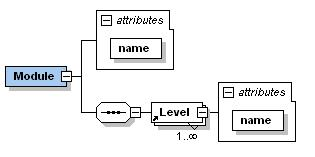
\includegraphics[width=10cm]{img/EsquemaXmlModulo.jpg}	
\caption{Esquema Xml del fichero module.xml}
\end{figure}

\lstinputlisting[title=Ejemplo de module.xml]{source/module.xml}

La etiqueta principal del fichero module.xml es Module. El atributo name indica el nombre del módulo y por cada sub-etiqueta Level, se está referenciado a un escenario del videojuego. El atributo name de la etiqueta Level, hace referencia al nombre del directorio que contiene su configuración.

\subsection{Niveles}

Hasta el momento se ha definido un módulo como una agrupación de escenarios, siendo éste, un concepto definido por la librería desarrollada. En el ámbito del videojuego es necesario ampliar las características del escenario, dando origen a un nuevo concepto, el de nivel, implementado por la clase \textbf{Level} y que extiende a la clase Scene.
\newline

Un nivel contiene nueva información como capturas de pantalla del escenario, referencias a ciertos elementos del juego como el pacman y los fantasmas, listado de cámaras utilizadas en distintos momentos del videojuego, etc.
\newline

La información del nivel es almacenada en un directorio, especificado en el fichero module.xml, que contiene los siguientes ficheros:
\begin{itemize}
\item \textbf{Image1.jpg}, una captura de pantalla del nivel con una resolución 64x64.
\item \textbf{Image2.jpg}, una captura de pantalla del nivel con una resolución 256x256.
\item \textbf{Texture.mesh} que contiene la información de la malla con todo el escenario.
\item \textbf{Music.mp3} con la melodía del escenario.
\item \textbf{video.mp4} con el vídeo de introducción del escenario.
\item\textbf{Level.xml:} que contiene la información asociada al nivel:
	\begin{itemize}
	\item Atributo name: nombre del nivel.
	\item Atributo description: descripción del nivel.
	\item Etiqueta Pacman\_Start: posición inicial del Pac-man.
	\item Etiqueta Ghost: información de los fantasmas  sobre su posición inicial en el escenario, la velocidad, su algoritmo y su malla.
	\item Etiqueta Small\_Pill: posición de cada pastilla del escenario.
	\item Etiqueta Wall: posición de cada bloque de pared del escenario.
	\end{itemize}
\end{itemize}

Es posible encontrarnos otros ficheros en el directorio, consecuencia de la definición de la malla. Estos ficheros pueden ser de tipo mtl e imágenes, los cuales  representan los materiales y texturas definidos en el escenario.

\begin{figure}[!h]
	\centering	
          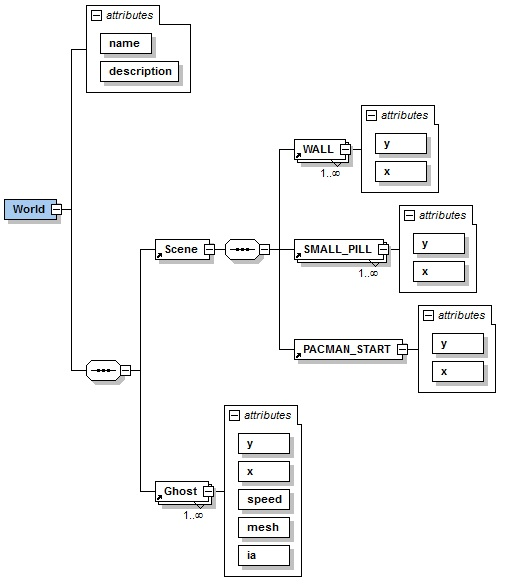
\includegraphics[width=14cm]{img/EsquemaXML_Nivel.jpg}
	\caption{Esquema xsd de level.xml}
\end{figure}

\lstinputlisting[title=Ejemplo de fichero level.xml]{source/level.xml}



\subsection{Lector de niveles}

Los ficheros level.xml son procesados por la aplicación para obtener instancias de la clase Level. El responsable de procesar estos ficheros es la clase \textbf{LevelReader}. Según se vayan procesando las etiquetas ocurrirán las siguientes acciones:
\begin{itemize}
\item Etiqueta \texttt{World}: se obtiene el nombre y descripción del nivel.
\item Etiqueta \texttt{Scene}: se crea la malla del escenario utilizando la clase MeshFileReader.
\item Etiqueta \texttt {Wall}: se crea una geometría AABB en función de las coordenadas X e Y de la etiqueta y se añade a la geometría del nivel.
\item Etiqueta \texttt{Small\_Pill}: se añade una nuevo vértice a la clase PathFinder ya que es un posible punto por el que los fantasmas y el Pacman pueden pasar y debe ser procesado en el algoritmo de Dijstra. También se añade una nueva pastilla al objeto PillsNetElement indicando su  posición.
\item Etiqueta \texttt{Pacman\_Start}: se añade una nuevo vértice a la clase PathFinder y se indica al elemento Pacman de la clase Level sus coordenadas y velocidad inicial.
\item Etiqueta \texttt{Ghost}: se añade un nuevo elemento al nivel de tipo GhostElement. En el constructor se indica su posición inicial en el escenario, su velocidad, si el comportamiento es aleatorio o de persecución y la referencia al Pacman, que es el elemento que ha de perseguir.
\end{itemize}

\begin{figure}[ch!]
\centering
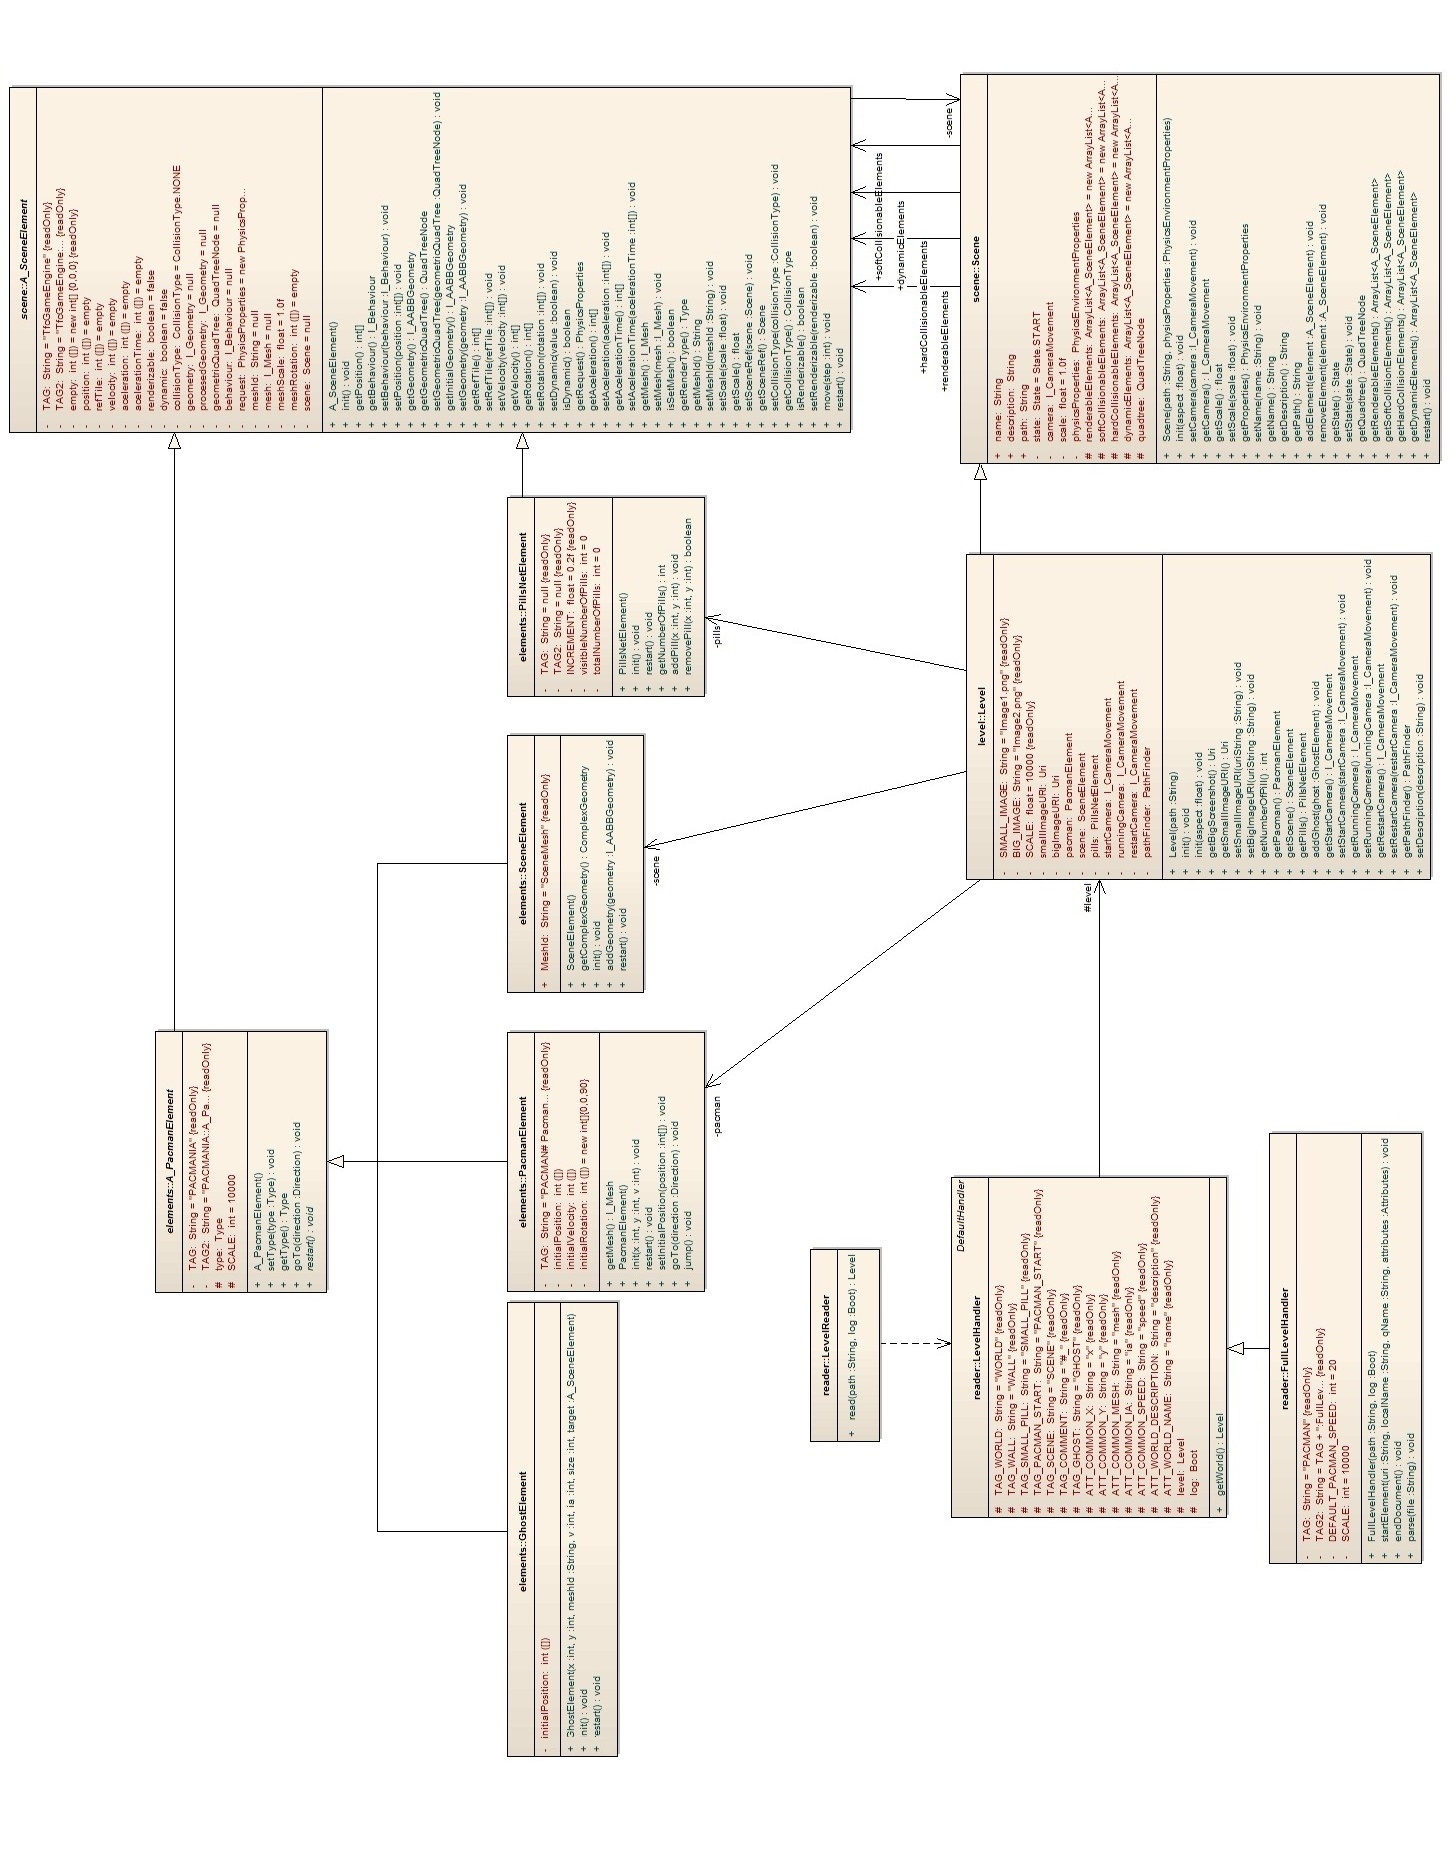
\includegraphics[width=15cm]{img/uml/LevelReader.jpg}	
\caption{Diagrama de clases de LevelReader}
\end{figure}

\begin{figure}[h!]
\centering
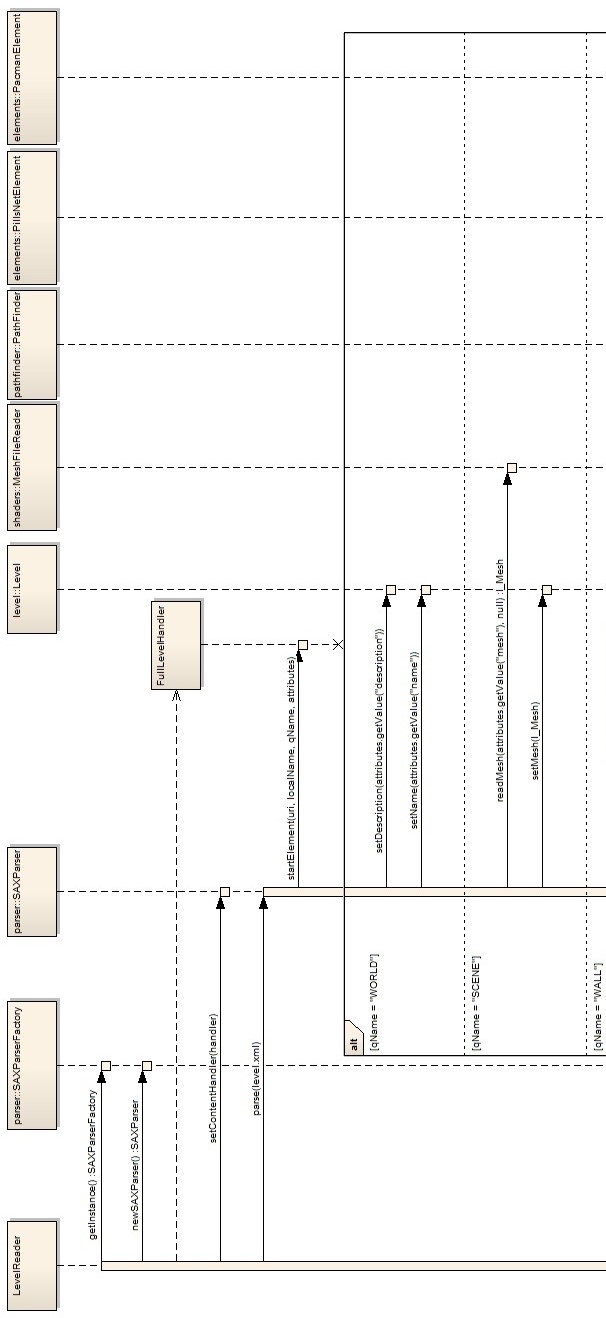
\includegraphics[height=19.5cm]{img/uml/LevelReaderRead1.jpg}	
\caption{Diagrama de secuencia para procesar el fichero level.xml (Parte 1)}
\end{figure}

\begin{figure}[h!]
\centering
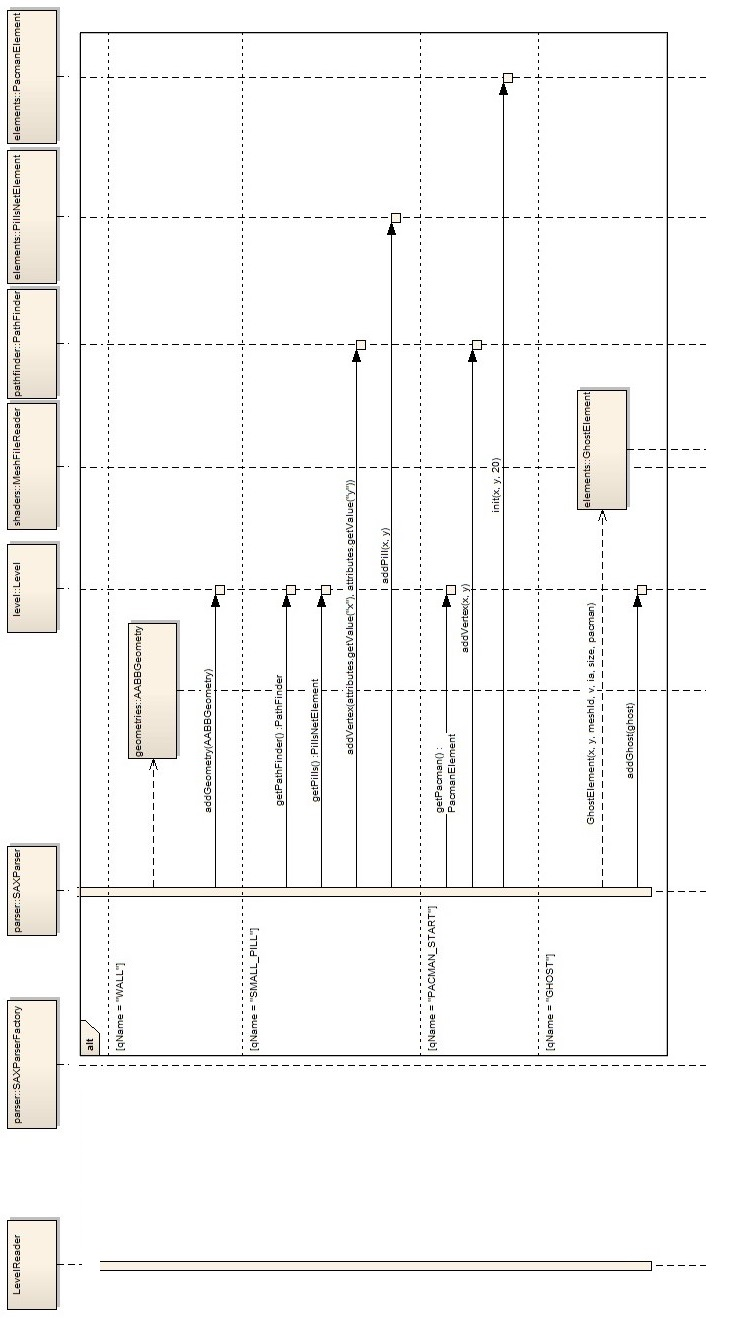
\includegraphics[height=19.5cm]{img/uml/LevelReaderRead2.jpg}	
\caption{Diagrama de secuencia para procesar el fichero level.xml (Parte 2)}
\end{figure}


\newpage




\subsection{Cámaras}

La clase Scene contiene una única cámara, a través de la cual se renderiza la escena. La clase Level contiene un listado de cámaras con distintos comportamientos. Según lo requiera el estado del videojuego se selecciona cuál de estas cámaras es la adecuada para renderizar la escena. 
En éste proyecto se han definido tres tipos de cámaras:

\begin{itemize}
\item \textbf{Cámara 1:} al comenzar la pantalla se realiza un zoom, acercándose al Pacman y a su vez inclinándose para percibir las tres dimensiones del escenario.

   \begin{minipage}{\linewidth}
         \centering
         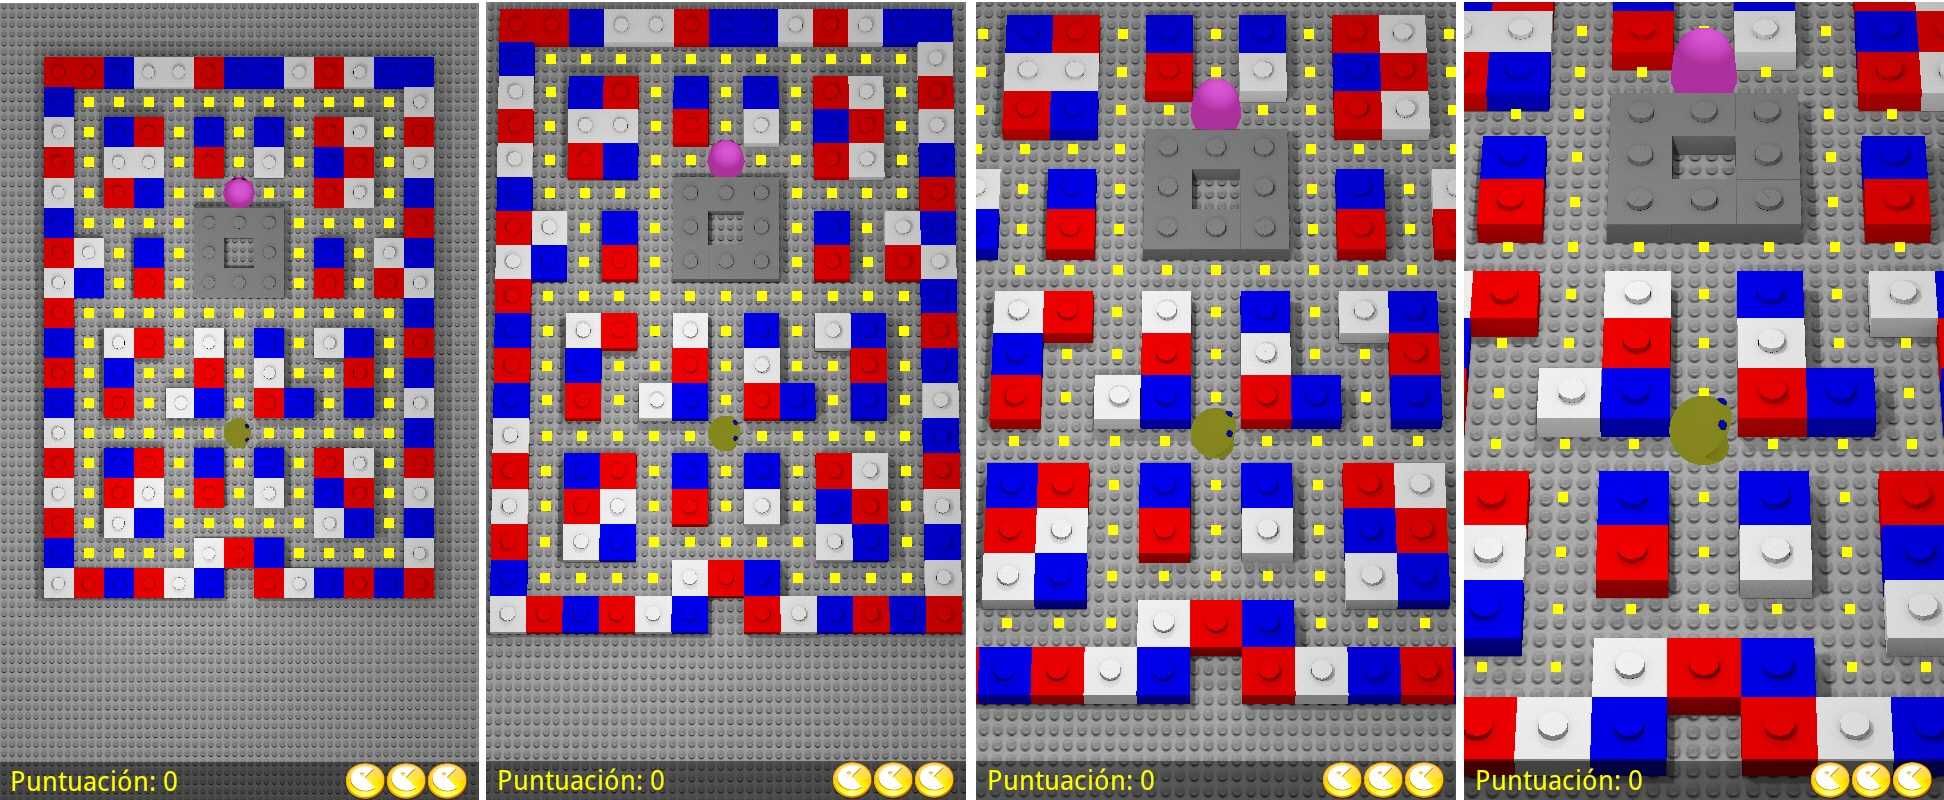
\includegraphics[width=13.5cm]{img/camaraZoom.jpg}	
    \end{minipage}

\item \textbf{Cámara 2:} cuando el Pacman ha sido capturado se realiza un giro de 360 grados mientras se aleja.

   \begin{minipage}{\linewidth}
         \centering
         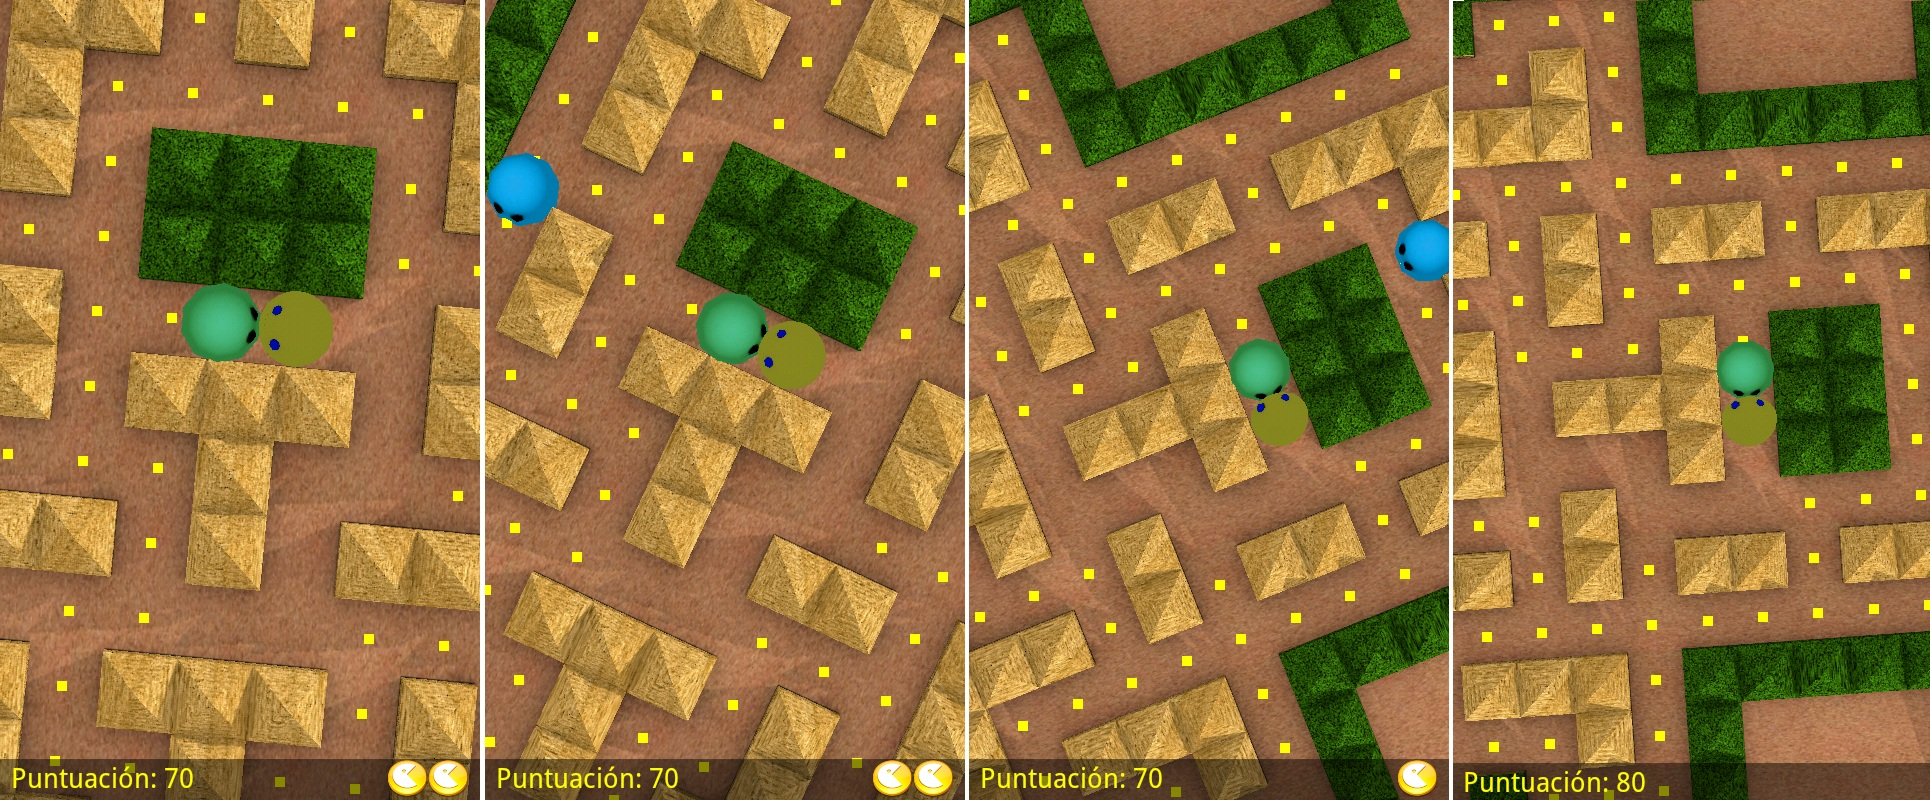
\includegraphics[width=13.5cm]{img/camaraRotate.jpg}	
    \end{minipage}

\item \textbf{Cámara 3:} es el habitual en la escena donde la cámara persigue al Pacman por el escenario desde una distancia fija.

\end{itemize}

\subsection{Pacman}

Dentro del directorio meshes se encuentra el directorio pacman, que contiene la malla del elemento Pacman. La característica a resaltar de este elemento radica en que es una animación, compuesta por dos mallas, una con la boca abierta y otra cerrada.

\begin{figure}[h]
\centering
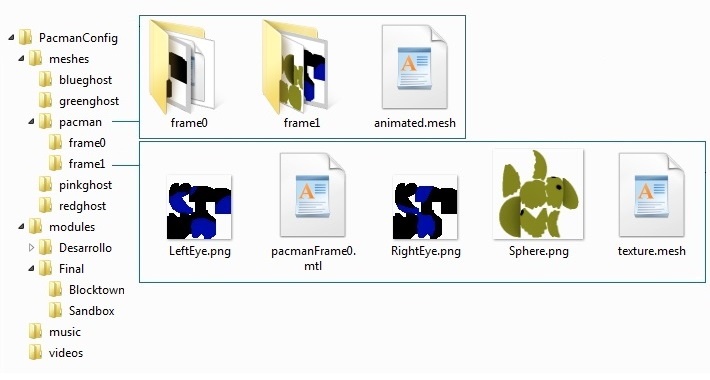
\includegraphics[width=14.5cm]{img/EstructuraPacman.jpg}	
\caption{Estructura del directorio del elemento Pacman}
\end{figure}

El fichero \textbf{animated.mesh} indica la secuencia de mallas que componen la animación. En cada línea se expresa el directorio que contiene la malla junto con el tiempo que se tiene que mostrar en milisegundos. 

\lstinputlisting[title=Fichero animasted.mesh del elemento Pacman]{source/animated.mesh}

Como se puede apreciar en el contenido del fichero, ambos frames se muestran 500 milisegundos y los nombres de frame0 y frame1 se corresponden con los directorios que contienen la información de las mallas. Al igual que la malla de BlueGhost, estos directorios contienen el fichero texture.mesh junto con los ficheros de materiales e imágenes descritos en él.




\subsection{Generación de mallas con Blender}

Entre todos los ficheros que se encuentran en el directorio PacmanConfig, resaltan debido a su complejidad los ficheros asociados con las mallas, por ese motivo han sido creados con la herramienta Blender y posteriormente dichos ficheros se leerán mediante la librería desarrollada.
\newline

Blender es una herramienta para generación de animaciones 3D tan compleja que existe un mercado laboral en torno a ella. Hay profesionales específicos para ciertas funcionalidades de la aplicación, por ejemplo, algunos se dedican a crear las mallas  y otros se especializan en cómo aplicarles las texturas. Obviamente, en el ámbito del proyecto tan sólo ha sido posible utilizar de forma somera, el potencial de la herramienta.
\newline

En el siguiente ejemplo se va a explicar cuál es el proceso seguido para generar la malla correspondiente a un fantasma del juego. Este proceso ha sido definido tras múltiples pruebas. En cada una de ellas se observaba el fichero final resultante de las acciones realizadas en el programa.

\begin{enumerate}
\item El primer paso, tras arrancar la aplicación, es crear una esfera tal y como se muestra en el gráfico.

   \begin{minipage}{\linewidth}
         \centering
          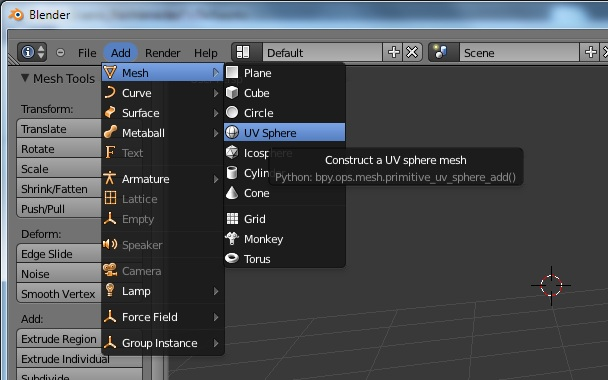
\includegraphics[height=4.9cm]{img/blender/blender1.jpg} 
	 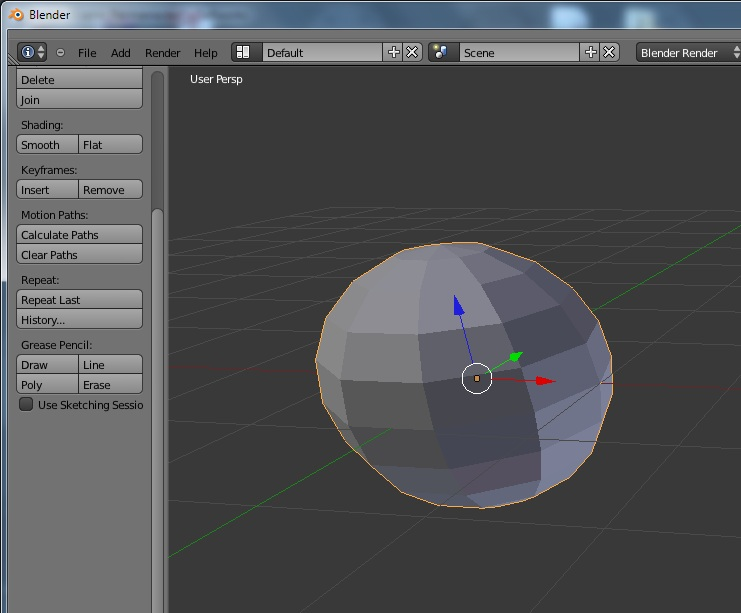
\includegraphics[height=4.9cm]{img/blender/blender2.jpg}
   \end{minipage}
 

\item Seleccionaremos sólo la mitad de la esfera. El resto de los vértices los borraremos, obteniendo media esfera.

   \begin{minipage}{\linewidth}
         \centering
          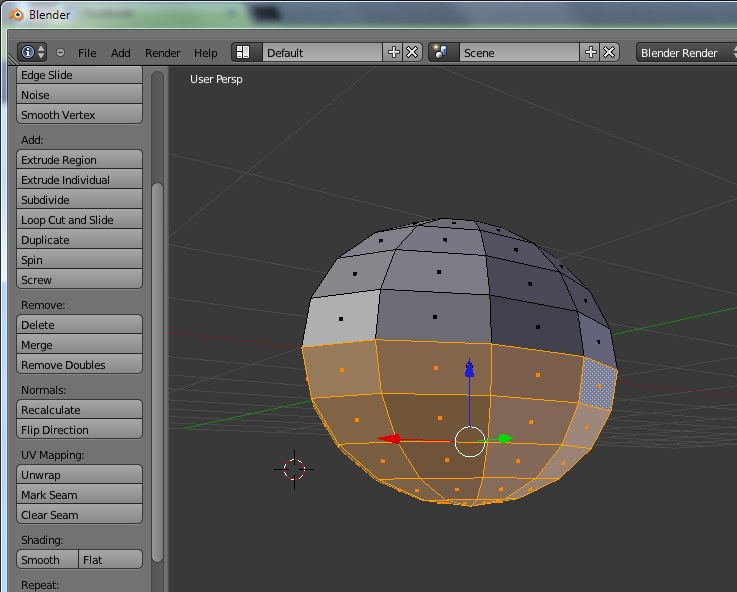
\includegraphics[height=4.9cm]{img/blender/blender3.jpg} 
	 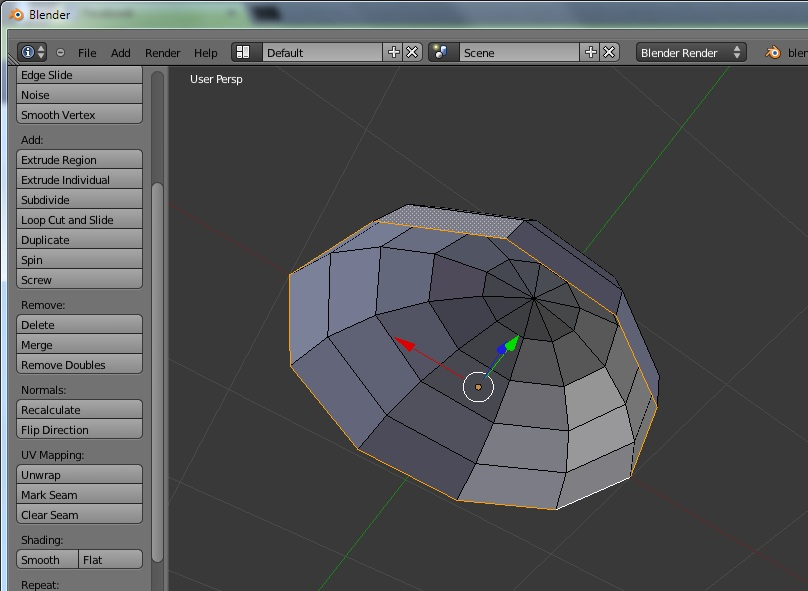
\includegraphics[height=4.9cm]{img/blender/blender4.jpg}
    \end{minipage}

\item El siguiente paso consiste en seleccionar las aristas de la base de la media esfera y moverlas para crear la figura final del fantasma.

   \begin{minipage}{\linewidth}
         \centering
          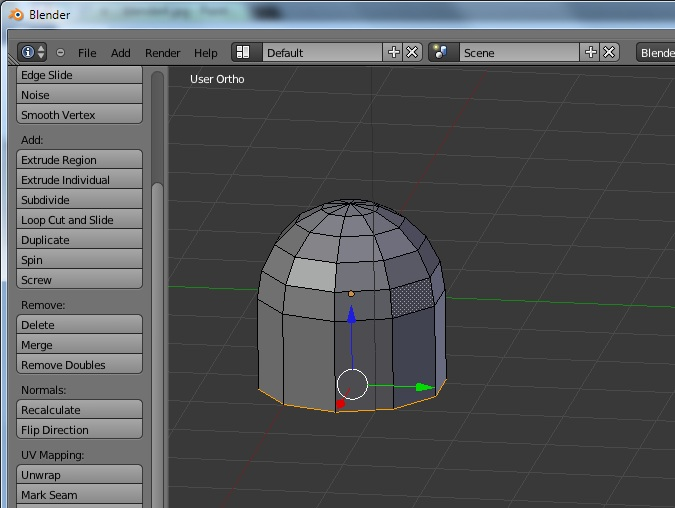
\includegraphics[height=4.9cm]{img/blender/blender5.jpg} 
    \end{minipage}

\item Aplicamos un material sobre la figura creada indicando el color de especulación, difusión y ambiental.

   \begin{minipage}{\linewidth}
         \centering
          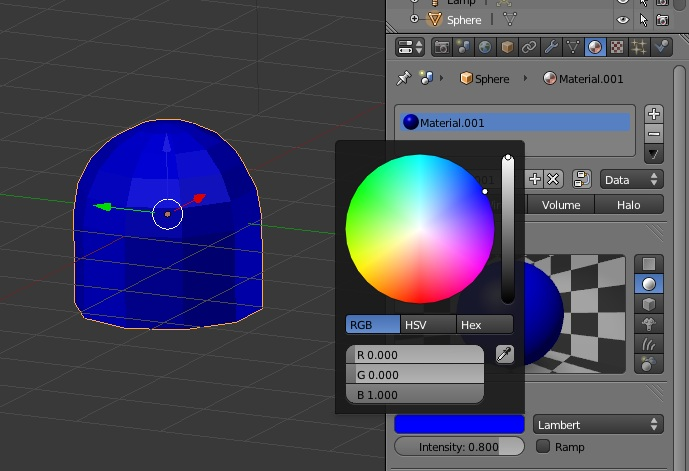
\includegraphics[height=4.9cm]{img/blender/blender6.jpg} 
    \end{minipage}

\item En la imagen aún se notan las cambios entre las distintas caras de la figura. Esto es debido a que el tipo de sombreado es Flat. Para que el salto sea homogéneo vamos a modificar el tipo de sombreado a Pong\footnote{El sombreado Phong es conocido por Smooth en las aplicaciones de diseño gráfico 3D}.

   \begin{minipage}{\linewidth}
         \centering
          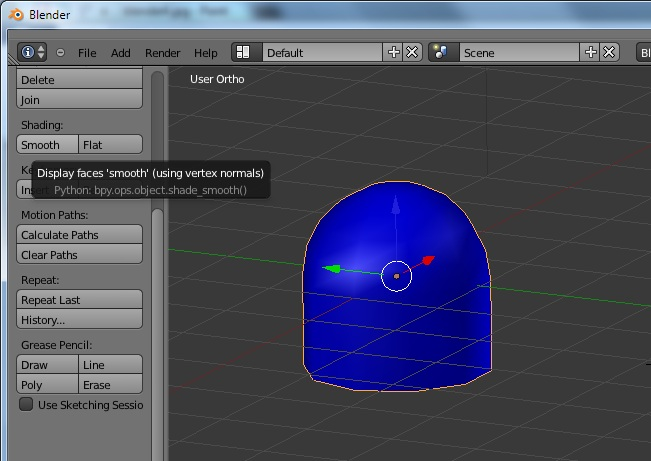
\includegraphics[height=5.5cm]{img/blender/blender7.jpg} 
    \end{minipage}

\item El siguiente paso es generar las texturas. Unwrap es el comando encargado de trasladar cada uno de los vértices de la figura sobre una imagen de color negro. En función de la complejidad de la malla que queramos mapear, es posible que encontremos situaciones donde la aplicación realiza el mapeo directamente u otras en las que hay que indicárselo manualmente, vértice a vértice.

   \begin{minipage}{\linewidth}
         \centering
          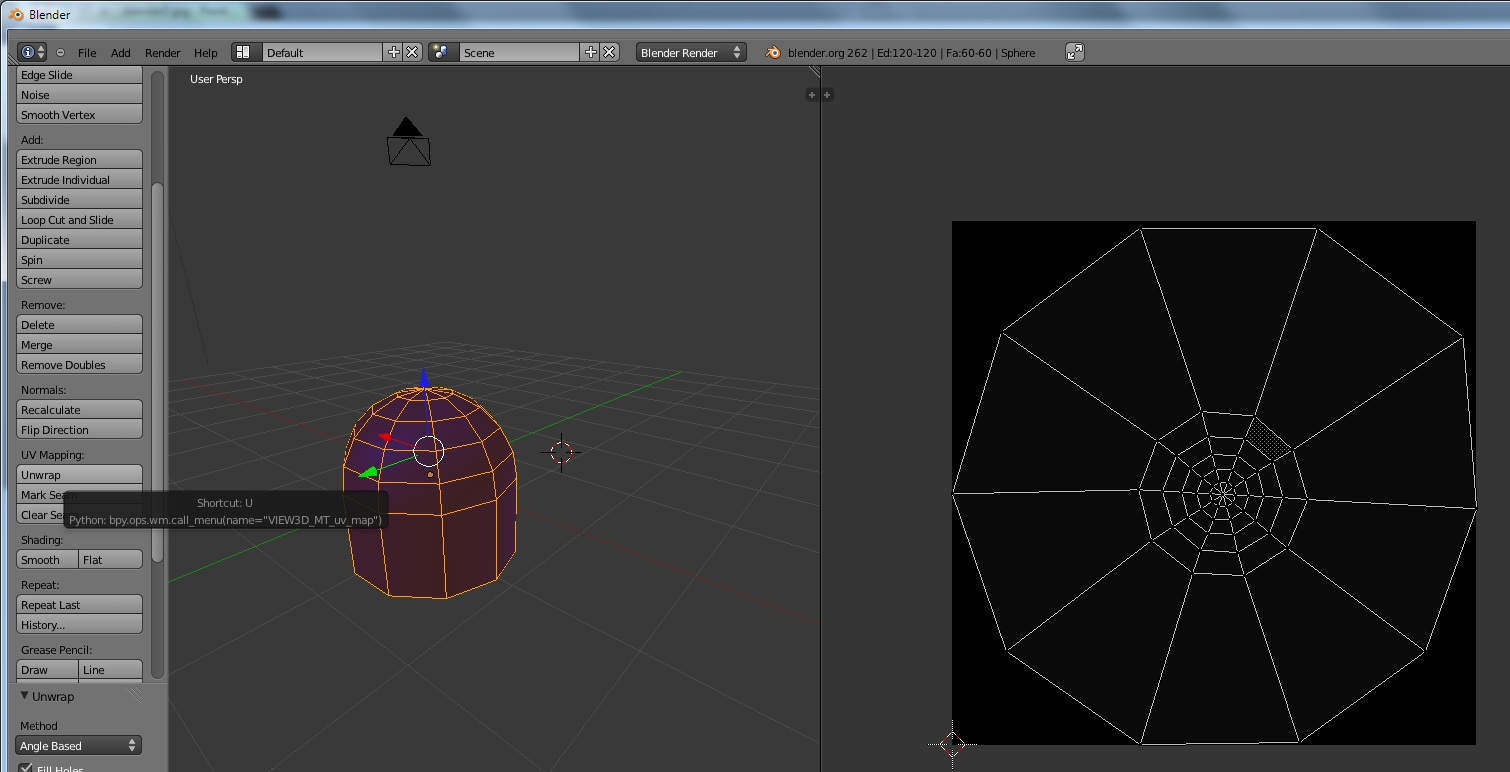
\includegraphics[height=5.5cm]{img/blender/blender8.jpg} 
    \end{minipage}

\label{textureBake}\item La imagen actual es negra y no refleja la realidad representada en la aplicación, por tanto, hemos de 'cocinar la escena'. Este concepto es conocido como \textbf{Texture bake} y consiste en aplicar un modelo de iluminación sobre los elementos de la escena y determinar su color final, atendiendo a los materiales y luces que la componen. En la captura de pantalla se puede ver el resultado de la operación y cómo se corresponde la cara seleccionada con la imagen. Esta correspondencia se trasladará al fichero obj mediante los vértices de la textura.

   \begin{minipage}{\linewidth}
         \centering
          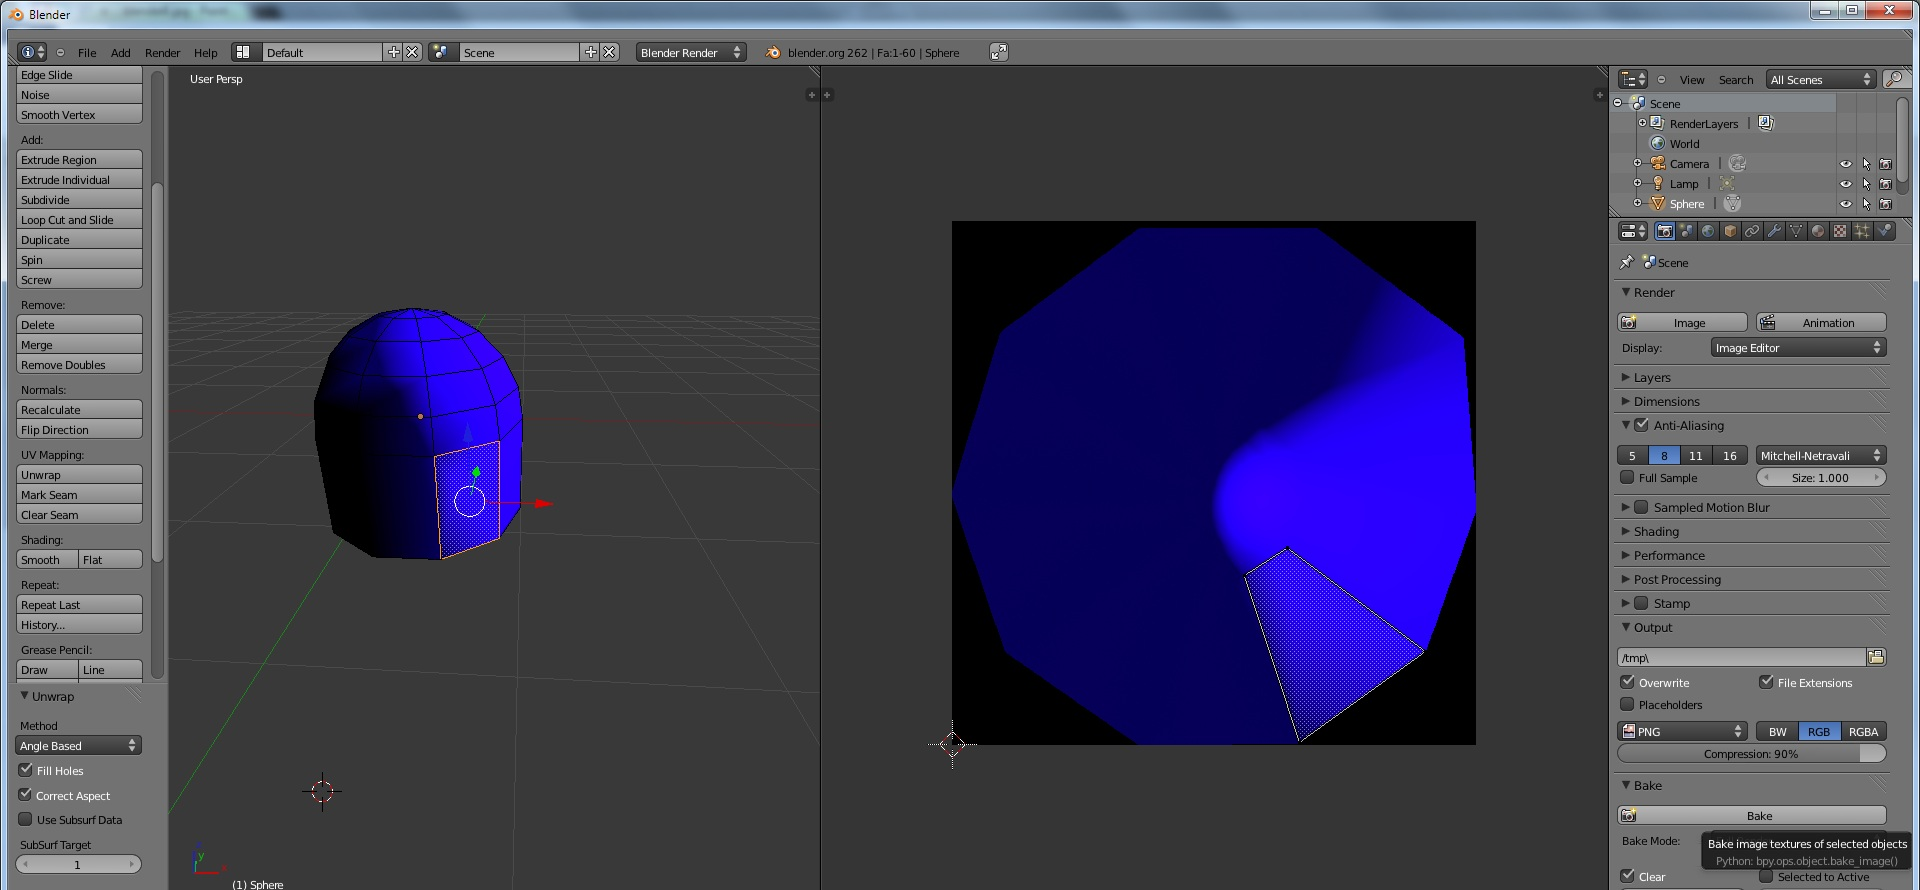
\includegraphics[height=6cm]{img/blender/blender9.jpg} 
    \end{minipage}

\item El último paso, consiste en exportar el trabajo realizado en Blender, al formato Wavefront. Es indispensable indicar las opciones de exportación correctas, de otro modo, la librería no sería capaz de renderizar correctamente la malla. Se ha de incluir las opciones de mapeo de texturas (Include UVs) y la exportación de las caras mediante triángulos (Triangule Faces).

   \begin{minipage}{\linewidth}
         \centering
         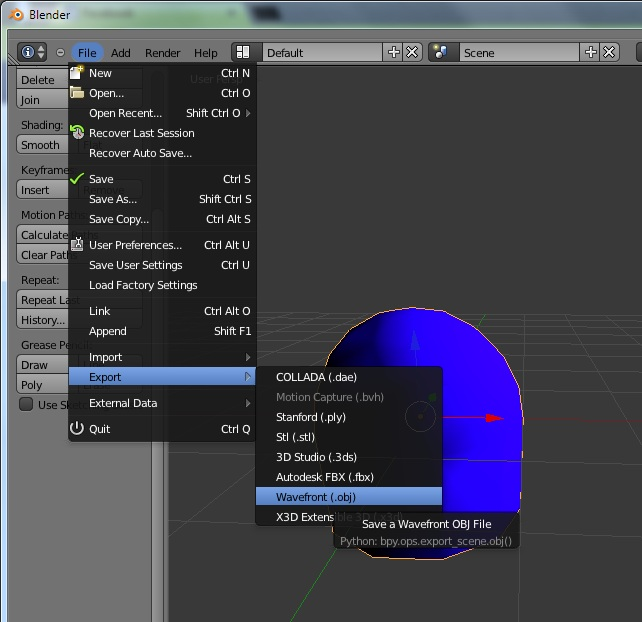
\includegraphics[height=5.8cm]{img/blender/blender10.jpg} 
         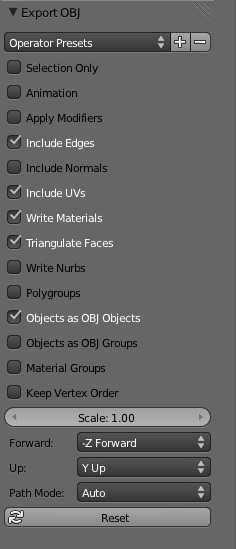
\includegraphics[height=5.8cm]{img/blender/blender11.jpg} 
    \end{minipage}

\item El resultado final es un fichero .obj que contendrá la información de la malla y hará referencia a un fichero .mtl con los materiales. En este caso, sólo existirá un material el cual hará referencia a la imagen cocinada.

   \begin{minipage}{\linewidth}
         \centering
          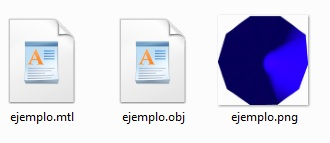
\includegraphics[height=3cm]{img/blender/blender12.jpg} 
    \end{minipage}

\end{enumerate}

\section{Actividad de arranque}

Una vez comprendida la estructura de directorio PacmanConfig, nos centramos en la actividad de arranque, implementada por la clase \texttt{Boot}. Esta actividad muestra las trazas de las comprobaciones realizadas al arrancar la aplicación. El primer mensaje indica que la aplicación se corresponde con un proyecto de fin de carrera y se muestra el nombre del alumno, el tutor, la universidad y facultad en la que se presenta. 
\newline

El segundo mensaje es el resultado de comprobar si existe el directorio donde está toda la configuración de la aplicación. Esta ubicación se establece en la propiedad \texttt{PacmanConfigPath}, cuyo valor por defecto es /sdcard/PacmanConfig. Por motivos de compatibilidad con otros dispositivos, es posible cambiar esta ruta en la actividad de preferencias del videojuego 
\newline

El siguiente paso es iniciar el gestor de música y cargar los sonidos que se van a utilizar durante el juego. En concreto los sonidos a cargar son \texttt{chomp} y \texttt{deatch}, los cuales se reproducen cuando existe una colisión entre el pacman-pastilla o pacman-fantasma respectivamente. Al cargar cada uno de los sonidos se mostrará una traza informativa.
\newline

A continuación se buscan las mallas comunes a todos los escenarios del juego, es decir, los correspondiente a los fantasmas y pacman. Todos ellos están contenidos en el subdirectorio meshes del PacmanConfig. Cada fichero que contiene una malla se procesará y cargará en la memoria utilizando la clase MeshFileReader, desarrollada en la librería del proyecto. Por cada fichero Wavefront que se vaya a procesar, ya sea obj o mtl, se mostrará un mensaje informativo.
\newline 

\begin{figure}[h!]
	\centering	  
	\subfloat{
	           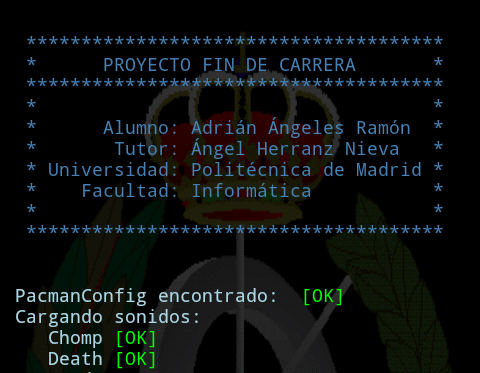
\includegraphics[width=6.5cm]{img/screenshot/boot1.png}
	}
	 \hspace*{0.5cm}
	\subfloat{
	          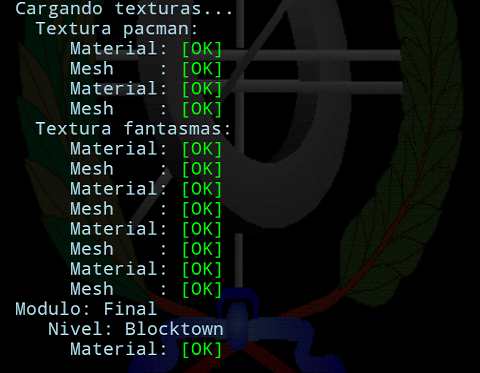
\includegraphics[width=6.5cm]{img/screenshot/boot2.png}
	}
	\caption{Actividad de arranque (Boot)}
\end{figure}

En relación al módulo, la propiedad module de la aplicación indica cuál es el módulo que ha de ser cargado entre los disponibles en el directorio \texttt{PacmanConfig}. Mediante la clase \textbf{ModuleHandler} se va a procesar el fichero module.xml y por cada uno de las referencias a un nivel, se utilizará la clase LevelReader para procesarlo.
\newline

Una vez completadas todas estas acciones, el contexto del videojuego estará cargado, se finalizará la actividad de arranque y se cargará la actividad principal.

\section{Actividad principal}
La actividad, implementada con la clase Pacman, está compuesta únicamente por el menú principal de la aplicación que permite realizar las siguientes acciones:
\begin{itemize}
\item \textbf{Comenzar juego:} inicia una partida para lo cual carga la actividad \texttt{StartGame}.
\item \textbf{Configuración:} muestra el menú con las opciones del videojuego contenido en la actividad \texttt{Preferences}.
\item \textbf{Marcadores:} inicia la actividad \texttt{Score} para ver las diez mejores puntuaciones obtenidas por los jugadores.
\item \textbf{Acerca de:} muestra una ventana de información indicando que la aplicación se trata de un proyecto y su información relacionada (autor,  tutor, año\ldots).
\item \textbf{Salir:} finaliza la actividad.
\end{itemize}

De fondo, al iniciar la actividad, se inicia la melodía ubicada en la ruta \texttt{PacmanConfig/music/Intro.mp3}.

\begin{figure}[h]
	\centering	
	\subfloat[Actividad Pacman]{
	          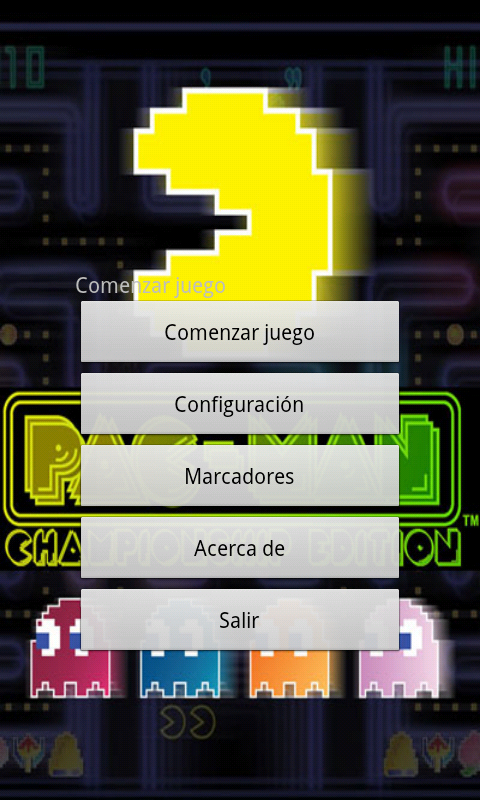
\includegraphics[width=5.5cm]{img/screenshot/pacman.png}
	}
	 \hspace*{0.5cm}
	\subfloat[Acerda de:]{
	          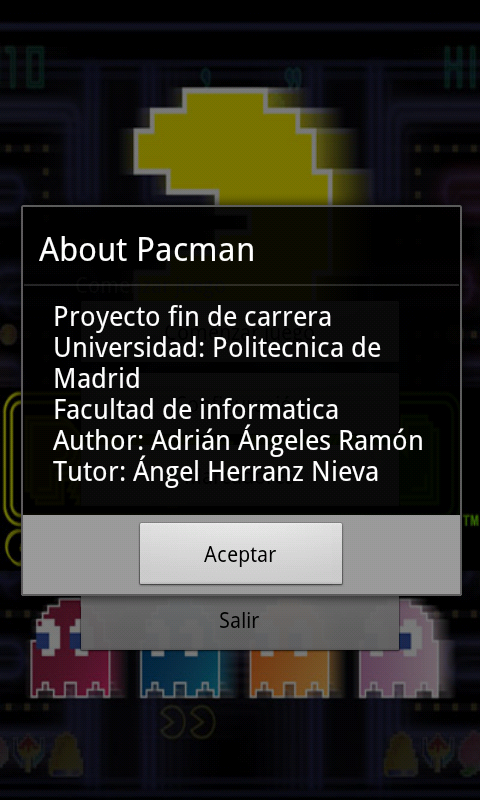
\includegraphics[width=5.5cm]{img/screenshot/about.png}
	}
\end{figure}

\section{Preferencias}

Desde la actividad principal, tras pulsar la opción de Preferencias, accedemos a la actividad \textbf{Preferences} que extiende de la clase nativa de Android  \textbf{PreferenceActivity} e implementa la interfaz \textbf{OnSharedPreferenceChangeListener}.
\newline

La clase PreferenceActivity permite crear pantallas de configuración de propiedades fácilmente, cargando a partir de un fichero xml las propiedades que se desean configurar. Además estas propiedades serán almacenadas automáticamente y de forma persistente.
\newline

La interfaz  OnSharedPreferenceChangeListener permite detectar cualquier cambio en las propiedades de la aplicación y actuar en consecuencia. El ejemplo más claro se produce al deshabilitar el sonido, provocando una invocación a la clase SoundEngine para que deje de reproducir cualquier tipo de sonido.
\newline

Las opciones a configurar en la aplicación son:
\begin{itemize}
\item \textbf{Sonido:} indicando si el sonido debe estar o no activo en el juego.
\item \textbf{PacmanConfig Path:} ubicación en la tarjeta SD donde se encuentra el directorio PacmanConfig.
\item \textbf{Directorio del módulo:} donde se indica cuál será el módulo a cargar en el videojuego de los existentes en el directorio PacmanConfig. Los módulos disponibles no se pueden cargar en un xml ya que se encuentran definidos en la estructura de directorios, por lo que dicho menú se crea de forma dinámica.
\end{itemize}
\lstinputlisting[title=Fichero xml de configuración setting.xml]{source/setting.xml}
\vspace{2mm}

En el fichero xml de configuración, podemos observar que no se muestra la opción del directorio del módulo. Esto es debido a que esta propiedad no es estática, depende de la información contenida en el directorio PacmanConfig, por ese motivo es cargada en tiempo de ejecución.

\begin{figure}[h!]
	\centering	
	\subfloat[Preferencias ]{
		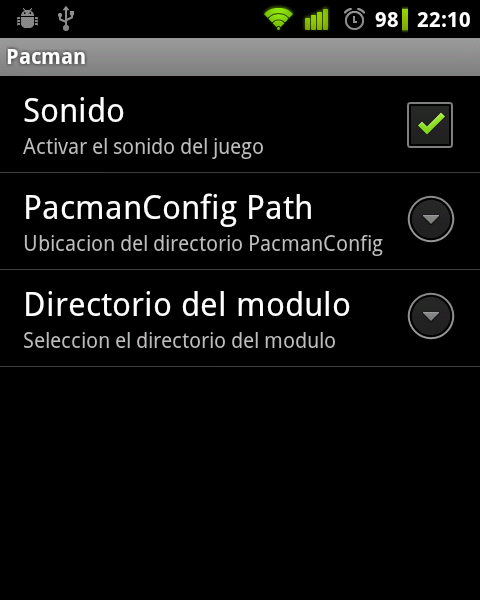
\includegraphics[width=5.5cm]{img/screenshot/preferences1.png}
	}
	 
	\subfloat[PacmanConfigPath]{
		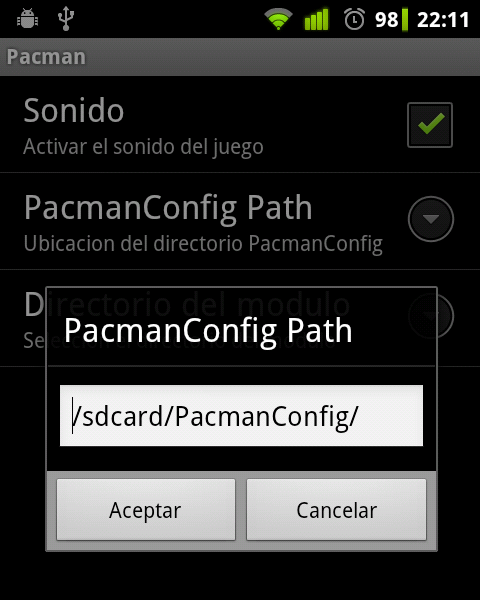
\includegraphics[width=5.5cm]{img/screenshot/preferences2.png}
	}
	\hspace*{0.5cm}
	\subfloat[Módulos]{
		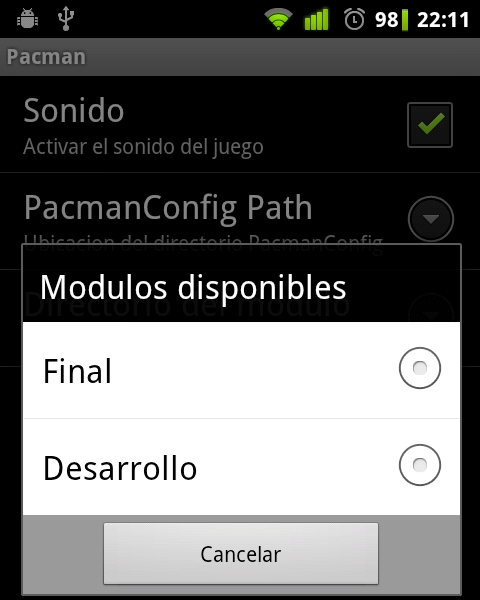
\includegraphics[width=5.5cm]{img/screenshot/preferences3.png}
	}	
\end{figure}


\section{Marcadores}

Al pulsar el botón \texttt{Marcadores} de la la actividad \texttt{Pacman}, se abre la actividad \textbf{Scores} que contiene un listado con las diez mejores puntuaciones. Por cada registro se indica, además de la puntuación, el nombre de la personas que lo consiguió, como se puede apreciar en la siguiente imagen.
\newline

Estas puntuaciones son almacenadas en una base de datos SQLite, sobre las cuales existe un soporte nativo en Android. Sus principales ventajas son la rapidez y bajo consumo de recursos. Por contra, no es posible realizar accesos de escritura de forma concurrente, debido a que almacena toda la información en un único fichero, que se bloquea al ser modificado.

\begin{figure}[h!]
	\centering	
	\subfloat[Marcadores]{
		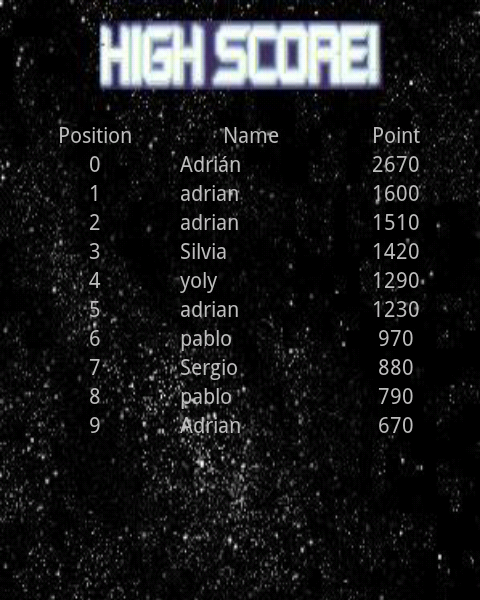
\includegraphics[width=5.5cm]{img/screenshot/score.png}
	}
	 \hspace*{0.5cm}
	\subfloat[Nuevo record]{
		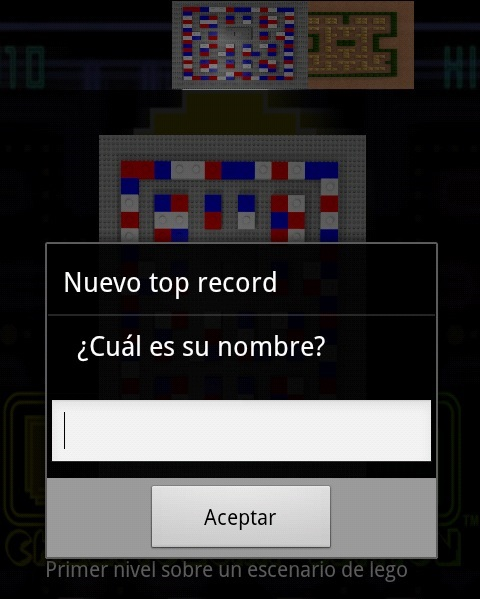
\includegraphics[width=5.5cm]{img/screenshot/toprecord.jpg}
	}
\end{figure}


\begin{figure}[!h]
	\centering	
	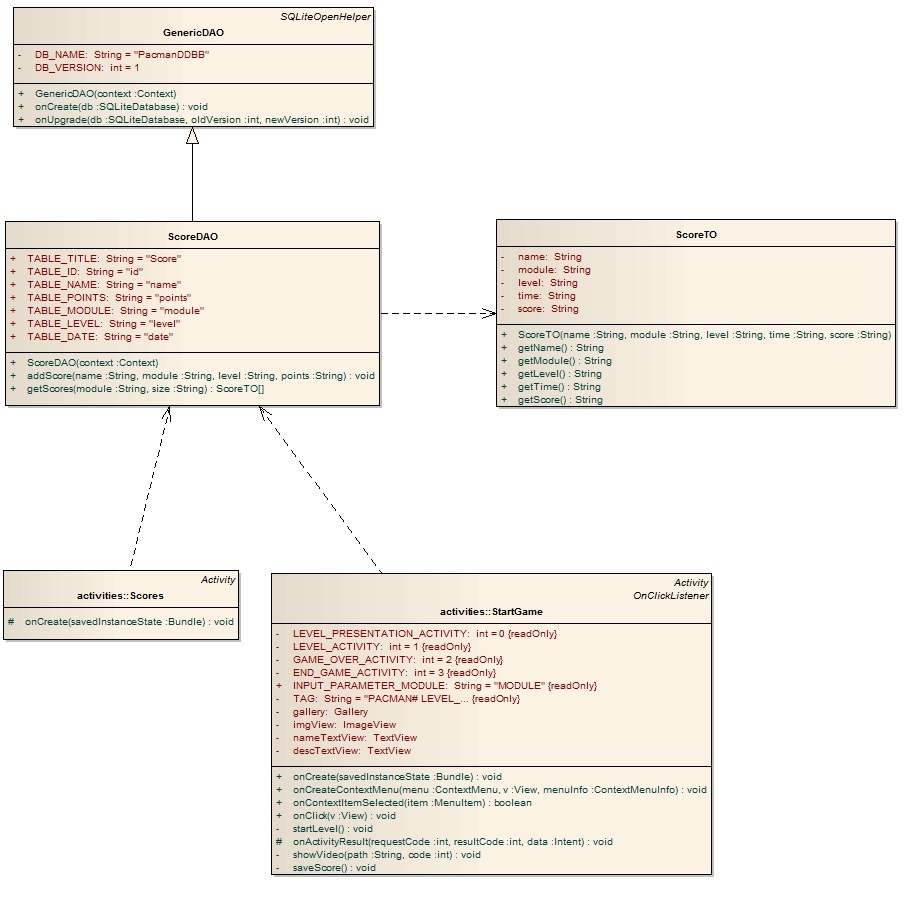
\includegraphics[width=15.5cm]{img/DiagramaClases_DAO.jpg}
	\caption{Diagrama de clases sobre SQLite}
\end{figure}

La clase \textbf{GenericDAO} extiende a la clase \textbf{SQLiteOpenHelper} y contiene el método \textbf{onCreate}. En este método se crea la base de datos, en el caso de que no exista,  en el espacio de disco reservada para la aplicación.
\newline

La clase \textbf{ScoreDAO} tiene la lógica requerida sobre la tabla \texttt{Score}. Permite el acceso de lectura para obtener las diez mejores puntuaciones y guardar puntuaciones nuevas. Estas funcionalidades son accedidas por la activididad Score y StartGame.

\lstinputlisting[title=Método OnCreate del GenericDAO]{source/genericdao.java}

\section{Actividad StarGame}

El objetivo inicial de esta actividad es seleccionar el escenario en el cual jugar, de los contenidos en el módulo cargado. Visualmente está compuesta en su parte superior con el componente \textbf{Gallery} de Android. Este componente gráfico permite mostrar un listado de imágenes, las cuales se corresponden con un escenario del videojuego. 
\newline

La parte inferior está compuesta por tres elementos gráficos que representan el nombre del escenario, una descripción del mismo y una imagen con mayor detalle del escenario. 
\newline

Al pulsar sobre cada imagen de la galería, la parte inferior cambia, mostrando los datos correspondientes al escenario seleccionado. También cabe destacar un cambió de música, el cual se corresponde con el nivel seleccionado.
\newline

La información relativa a cada nivel se encuentra almacenada en el contexto de la aplicación y ha sido cargada previamente en la actividad \texttt{Boot}.
\newline

Volviendo sobre el ejemplo del escenario SandBox, el nombre y la descripción del escenario estaría contenida en los atributos del fichero \texttt{level.xml}, las imágenes mostradas se corresponden con {Image1.png} e \texttt{Image2.png} y la música con el fichero \texttt{music.mp3}.
\newline
 
\begin{figure}[h!]
	\centering	
	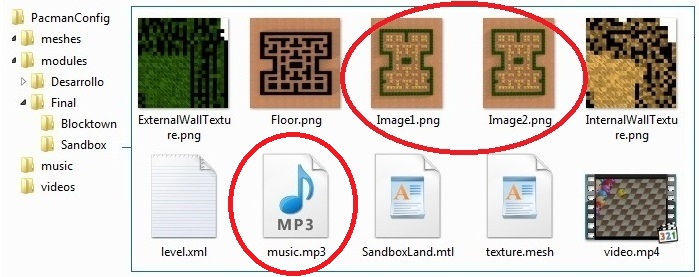
\includegraphics[width=15cm]{img/Sandbox2.jpg}
	\caption{Configuración escenario SandBox}
\end{figure}

Una vez seleccionado un escenario, si pulsamos sobre la imagen central del escenario en el que queremos jugar, comienza el objetivo principal de esta actividad, que consiste en coordinar la sucesión de escenarios y vídeos.
\newline

\begin{figure}[h!]
	\centering	
	\subfloat{
		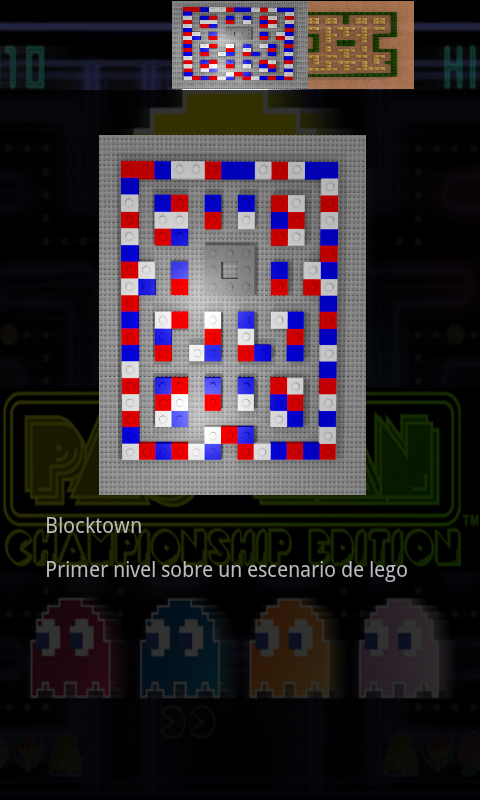
\includegraphics[width=5.5cm]{img/screenshot/game1.png}
	}
	 \hspace*{0.5cm}
	\subfloat{
			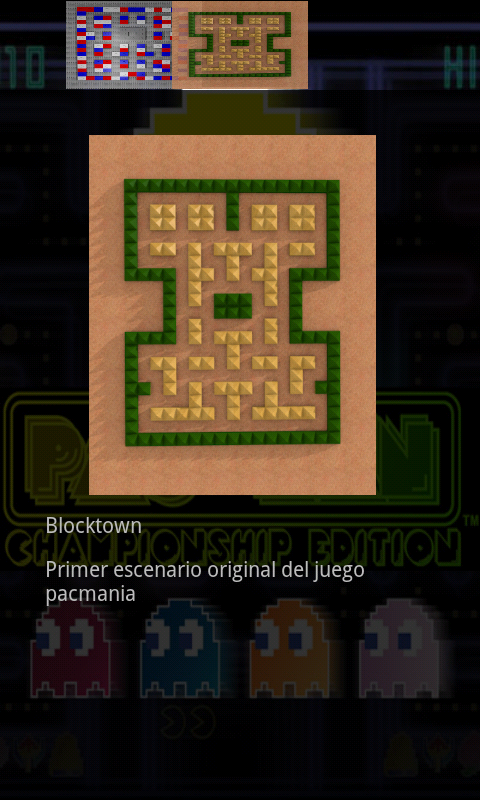
\includegraphics[width=5.5cm]{img/screenshot/game2.png}
	}
	\caption{Captura de pantalla de la actividad StartGame}
\end{figure}

Tras haber seleccionado el escenario en el cual queremos jugar, se mostrará el vídeo asociado a dicha pantalla, que está almacenado con el nombre \texttt{video.mp4} en el directorio raíz del mismo. Una vez concluido el vídeo, se creará una nueva actividad de tipo \textbf{StartLevel} que cargará el escenario seleccionado para jugar en él.
\newline

La actividad StartLevel puede concluir de dos formas, habiendo finalizado el escenario o cuando el usuario pierde todas las vidas. La actividad \texttt{StartGame} ha de identificar cuál es el motivo de cierre de la actividad \texttt{StartLevel} y actuar en consecuencia ya que:
\begin{itemize}
\item Si el usuario ha perdido todas las vidas de las que dispone, se ha de mostrar el vídeo \texttt{GameOver.mp4} ubicado en la carpeta \texttt{videos} del directorio principal.
\item Si el usuario ha finalizado con éxito la pantalla, en caso de no ser la última se ha de proceder a cargar el vídeo del siguiente escenario. Si no existen mas pantallas se ha de mostrar el vídeo \texttt{GameComplete.mp4} ubicado en el mismo lugar que \texttt{GameOver.mp3}.
\item Tras mostrarse el vídeo de un escenario, ha de crearse una actividad \texttt{StartLevel} correspondiente al vídeo mostrado en pantalla.
\item Tras finalizar el vídeo de \texttt{GameComplete.mp4} o \texttt{GameOver.mp4} se comprobará si la puntuación obtenida esta entre las diez mejores del juego. Si esto ocurre se solicitara al usuario introducir su nombre para grabarlo en el histórico.
\end{itemize}

\section{Actividad StartLevel}

A nivel visual, la actividad \textbf{StartLevel} está compuesta por dos componentes gráficos:
\begin{itemize} 
\item El primero de ellos ocupa toda la pantalla y se corresponde con el componente de Android \textbf{GLSurfaceView}. Es responsable de capturar los eventos producidos sobre la pantalla y contiene en su interior un render de OpenGL. El render a utilizar es el \textbf{PacmanRenderEngine}, el cuál extiende el desarrollado en la librería del proyecto. 

\item El segundo es un layout situado en la parte  inferior de la pantalla. Contiene el número de vidas del jugador y la puntuación actual.
\end{itemize}

\begin{figure}[h]
	\centering	
	\subfloat[BlockTown]{
		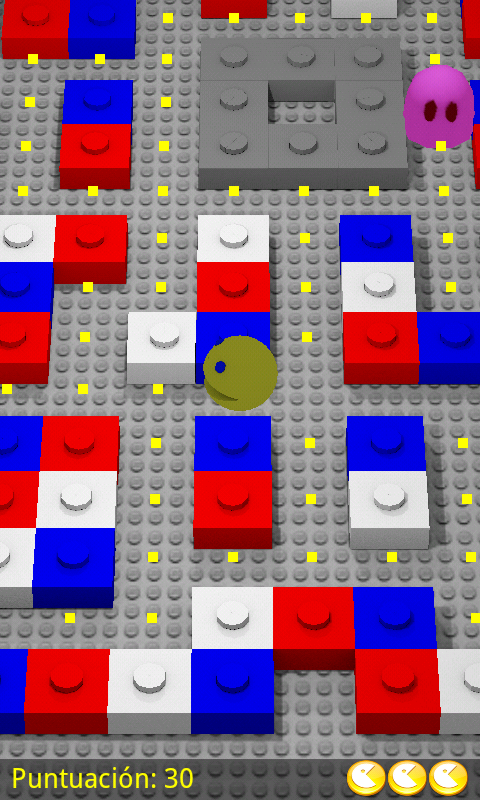
\includegraphics[width=5.5cm]{img/screenshot/level1.png}
	}
	\hspace*{0.5cm}
	\subfloat[Sandbox]{
		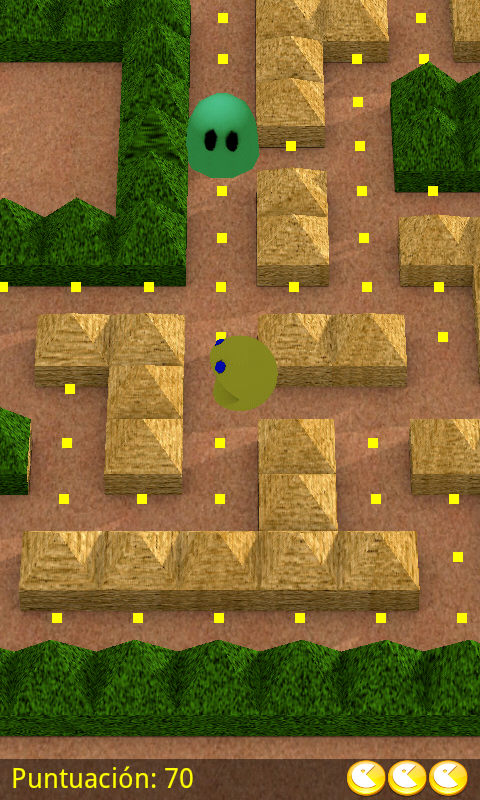
\includegraphics[width=5.5cm]{img/screenshot/level2.png}
	}
	\caption{Captura de pantalla de los escenarios desarrollados}
\end{figure}

La forma de interactuar con el componente GLSurfaceView se basa en la detección de movimientos del dedo sobre la pantalla. El método \textbf{onTouchEvent} es invocado al detectar un movimiento sobre la pantalla táctil, ofreciéndonos información sobre la posición que se está presionando y el tipo de evento entre los cuales están:
\begin{itemize}
\item ActionDown: ocurrido cuando el usuario presiona con el dedo la pantalla.
\item ActionUp: ocurrido cuando el usuario despega el dedo de la pantalla.
\end{itemize}

Al analizar la secuencia de eventos provocados por la pantalla táctil, se realizarán las siguientes acciones:
\begin{itemize}
\item Al desplazar el dedo de izquierda a derecha, estará indicando que el Pacman ha de desplazarse hacia la derecha, en cuanto sea posible. 
\item Al desplazar el dedo de derecha a izquierda, estará indicando que el Pacman ha de desplazarse hacia la izquierda, en cuanto sea posible.
\item Al desplazar el dedo de arriba a abajo, estará indicando que el Pacman ha de desplazarse hacia abajo, en cuanto sea posible.
\item Al desplazar el dedo de abajo a arriba, estará indicando que el Pacman ha de desplazarse hacia arriba, en cuanto sea posible.
\item Si se presiona la pantalla con el dedo y seguidamente, sin desplazarlo, se levanta, el Pacman saltará.
\end{itemize}

El elemento Pacman, cuyo comportamiento se basa en la clase PacmanBehaviour, intentará moverse en la dirección indicada, cuando la posición actual del Pacman sobre el escenario lo permita.
\newline

Es posible usar el trackball para mover al Pacman, siempre y cuando el smartphone disponga de de uno. Además es posible pausar el videojuego mediante el botón menú del móvil. Cuando el videojuego esté en pausa, cambiará la tonalidad a tonos sepia como se puede ver en la siguiente imagen.

\begin{figure}[h]
	\centering	
	\subfloat[Sin pausa]{
		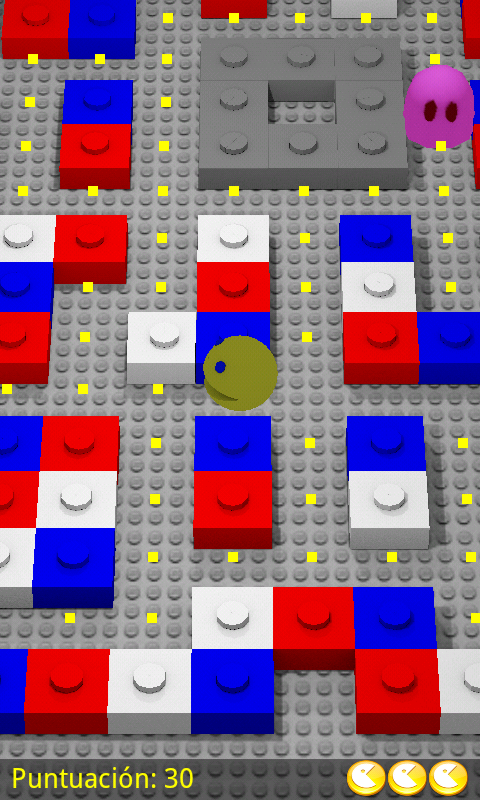
\includegraphics[width=4cm]{img/screenshot/level1.png}
	}
	\subfloat[Con pausa]{
		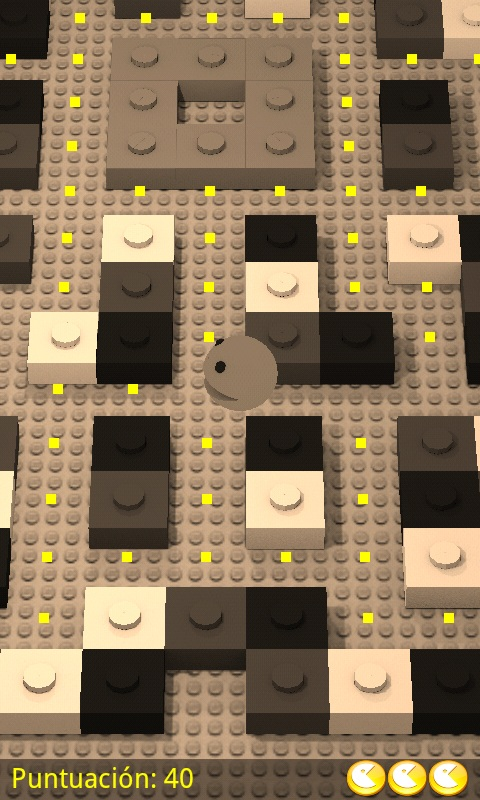
\includegraphics[width=4cm]{img/pausa.jpg}
	}
\end{figure}


\subsection{PacmanRenderEngine}

Ahora que comprendemos cómo es posible dirigir el comportamiento del Pacman, hemos de centrarnos en la clase PacmanRenderEngine. Esta clase se adapta a las necesidades concretas del videojuego, extendiendo el GameEngine e implementando las operaciones de preRender mencionada en el capítulo anterior.
\newline

Antes de cada pasada del bucle principal del juego, se ejecuta la operación \texttt{preRender}, sobre la cual se ha implementando la siguiente máquina de estados:
\begin{figure}[h]
	\centering	
	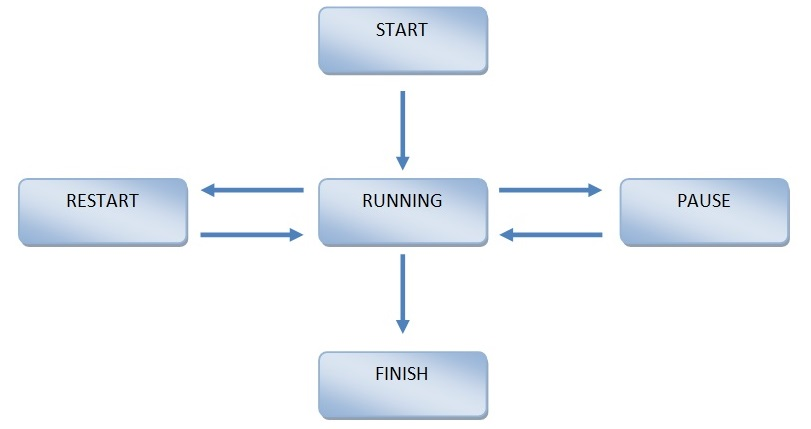
\includegraphics[width=12.5cm]{img/PacmanEngineRenderStates.jpg}
\end{figure}

\subsubsection{El estado Start}

Este estado transcurre desde que se inicia el nivel hasta que la cámara inicial o cámara 1, ha completado su recorrido. Realiza un acercamiento hasta la posición del Pacman, junto con una ligera inclinación, pudiendo apreciar las tres dimensiones del juego. Una vez completado el movimiento de la cámara se cambia al estado \texttt{Running}.
 
\subsubsection{El estado Running}
En este estado los elementos del juego empiezan a moverse sobre el escenario, la cámara ha sido sustituida por la cámara 3, que persige al Pacman. Tras cada iteración se comprueba si existen colisiones con los distintos elementos del juego actuando en consecuencia.
\newline

Si la colisión se produce sobre uno de los fantasmas, se  invoca al motor de sonidos para ejecutar el sonido death, se quita una vida al jugador y el estado se cambia a \texttt{Restart}. 
\newline

Si la colisión es con una pastilla, implica modificar el marcador, ejecutar el sonido chomp y actualizar el elemento PillsNetElement, para que no renderize la pastilla. 
\newline
Finalmente se ha de verificar si existe alguna otra pastilla sobre el escenario. En el caso de haber sido la última, se procede a cambiar al estado \texttt{Finish}.




\subsubsection{El estado Restart}
Al iniciar este estado, se modifica la cámara para que realice un efecto de giro de 360 grados. La duración de este estado coincide con la duración de la animación de dicha cámara. Al finalizar la animación, si el usuario aún continúa teniendo vidas, cambia al estado \texttt{Start}, en caso contrario, la partida debe finalizar, yendo al estado \texttt{Finish}.
\newline

Antes de poder volver al estado \texttt{Start} será necesario volver a reiniciar las posición tanto del elementos Pacman como de los fantasmas que componen la escena.

\subsubsection{El estado Pause}
Durante este estado \texttt{Running} es posible que el usuario presione la tecla de pausa, cambiando de forma automática al estado \texttt{Pause}. Al volver a presionar sobre la tecla de pausa, vuelve automáticamente al estado de \texttt{Running}. 
\newline

Durante este estado, el motor de sonido ha sido parado y se produce un cambio en un parámetro del render, modificando la iluminación de la escena a tonos sepia. Estos cambios son revertidos al salir del estado.

\subsubsection{El estado Finish}
Este es él último estado del escenario mediante el cual se cierra la actividad, volviendo a la actividad \texttt{StartGame}, la cual atendiendo a la forma en que finalizo el escenario, decidirá la siguiente acción, como ya se explicó previamente.

\subsection{Comunicación entre actividad y render}

Por último, cabe resaltar la problemática debida a que la actividad \texttt{StartLevel} es ejecutada en un thread principal y el renderer de \texttt{OpenGL} en otro. Al actualizar desde el método \texttt{preRender}, la puntuación y el número de vidas de la partida en pantalla,  se produce un error de privilegios, provocado por estar accediendo desde el thread de OpenGL. Para evitar esta situación, se envían mensajes entre los distintos thread usando la clase \textbf{Message} de Android. Cuando el thread de la actividad recibe dicho mensaje, accede a la clase GameContext para recuperar la puntuación y el número de vidas, para después, actualizarla en pantalla.
\newline

Para que la actividad detecte el mensaje, ha de contener una propiedad publica de tipo \texttt{Handler}, a partir de la cual, el thread de OpenGL, enviará el evento.

\lstinputlisting[title=Envió del mensaje desde la clase PacmanRenderEngine]{source/msg-pacmanrender.java}

\lstinputlisting[title=Captura del mensaje en la clase StartLevel]{source/msg-startlevel.java}
